\chapter{The CTS Spec: How You Tell the Tool to Build the Clock}

\begin{tldr}
\begin{itemize}
  \item \textbf{Last chapter:} DEF was the snapshot of where everything lives. \textbf{This chapter:} the CTS spec is the instructions for how the biggest single set of those things (the clock network) gets built between post-place and post-route DEF.
  \item The \textbf{CCOPT spec} is a Tcl/CSV artifact that tells Innovus the per-clock targets: \textbf{skew, latency, max transition, NDR, skew groups, useful-skew limits}, and mesh boundaries.
  \item Clock nets do not route like data nets. They get \textbf{non-default routing rules (NDR)} for shielding and width, and they get \textbf{balanced} across endpoints inside a skew group.
  \item Get the spec wrong and you spend a week chasing a clock spine that ate three M5 tracks too many or a generated clock that drifted 60~ps from its master.
\end{itemize}
\end{tldr}

\begin{hook}
Open post-place DEF and post-route DEF side by side. Same netlist, you would think, with wires filled in. Except the cell count grew by roughly five percent, every flop has a new buffer chain feeding it, and the clock nets look nothing like what synthesis handed you. Something ran in between that cloned hundreds of buffers, picked routing layers the data nets are not allowed to touch, and balanced arrival times to within ten picoseconds at thousands of sinks. What did that thing read to know what to do?
\end{hook}

\section{What the CTS Spec Actually Is}

The \textbf{CTS spec} (in Innovus, the \textbf{CCOPT spec}) is a small text file (Tcl directives plus an optional CSV) that tells \texttt{ccopt\_design} how to build and balance the clock network. It is not RTL, it is not constraints in the SDC sense, and it is not floorplan. It is a \textbf{per-clock recipe}: for each clock root, what is the target latency, what is the target skew, which other clocks share its skew budget, what routing rule do the segments use, and where (if anywhere) does the network transition from a tree to a mesh.

The Synopsys ICC2 equivalent lives inside \texttt{clock\_opt} and a \texttt{.ccopt}-equivalent CSV; the vocabulary is nearly identical, the keywords differ.

\begin{keyidea}
The CTS spec is the \textbf{only place in the flow where you express clock-network intent declaratively}; everything else (placement, route, sign-off) just reacts to the tree CCOPT builds from it.
\end{keyidea}

A realistic CCOPT spec snippet looks like this:

\begin{lstlisting}[style=eda, caption={Excerpt from a CCOPT spec for a two-clock subsystem.}, label={lst:ccopt-spec}]
# ---- global CTS knobs ----
set_ccopt_property buffer_cells       {CKBUFM8 CKBUFM12 CKBUFM16}
set_ccopt_property inverter_cells     {CKINVM8 CKINVM12 CKINVM16}
set_ccopt_property clock_gating_cells {CKLNQM8 CKLNQM12}
set_ccopt_property target_max_trans   80ps
set_ccopt_property use_inverters      true

# ---- per-clock targets ----
create_ccopt_clock_tree clk_core -source [get_db pins CLKGEN/clk_core]
set_ccopt_property -clock_tree clk_core target_skew    50ps
set_ccopt_property -clock_tree clk_core target_latency 350ps
set_ccopt_property -clock_tree clk_core routing_rule   NDR_2W2S_M5M6

create_ccopt_clock_tree clk_io   -source [get_db pins CLKGEN/clk_io]
set_ccopt_property -clock_tree clk_io   target_skew    75ps
set_ccopt_property -clock_tree clk_io   routing_rule   NDR_1W2S_M4M5

# ---- skew groups ----
create_ccopt_skew_group -name core_grp \
    -sources {CLKGEN/clk_core CLKGEN/clk_core_div2}
create_ccopt_skew_group -name io_grp   -sources {CLKGEN/clk_io}
create_ccopt_skew_group -name dft_grp  -sources {CLKGEN/clk_dft}

# ---- run it ----
ccopt_design -cts
\end{lstlisting}

Four things are happening here. The first block sets the \textbf{cell palette} CCOPT is allowed to clone from. The second creates a tree per clock root with its own skew and latency targets. The third declares \textbf{which clocks share a balance budget}. The fourth runs the engine.

\begin{hook}
A CCOPT spec is the \textbf{conductor's score} for the orchestra of flops. Skip the part that says ``violins and violas share a downbeat'' and the section drifts a quarter note; in silicon a quarter note is 60~ps of skew and your launch-capture pair misses by an entire setup margin.
\end{hook}

\section{Clock Skew Groups}

\textbf{Skew} is the difference in clock arrival time between two endpoints. CCOPT will spend buffers and routing to flatten skew, but only \emph{within a skew group}. Two clocks in different groups are allowed to drift relative to each other because the tool assumes you do not have any path that closes timing between them.

You put clocks in the same skew group when \textbf{paths exist between their endpoints} (synchronous CDC, generated clocks of a common master, mux-selected clocks that converge on the same flops). You keep them in separate groups when the domains are \textbf{truly asynchronous} (handled by a CDC synchronizer) so CCOPT does not waste buffers trying to flatten a difference no timing path cares about.

\begin{gut}
You have \texttt{clk\_core} at 800~MHz and \texttt{clk\_core\_div2} at 400~MHz, generated from \texttt{clk\_core} by a divide-by-two flop. A handful of paths cross from div2 flops back to core flops. Same group or different?
\gutans{Same group. The two clocks share endpoints, and you need their insertion delays balanced so the cross-domain paths close at sign-off. If you leave the divider in its own group, CCOPT balances the div2 tree to itself and the divider output drifts ~40--80~ps from the core tree, blowing the cross-domain setup checks even though the RTL is perfectly synchronous.}
\end{gut}

\subsection*{Worked numbers: three clocks, two groups}

Take three clocks on a small subsystem:

\begin{center}
\begin{tabular}{lll}
\textbf{Clock} & \textbf{Frequency} & \textbf{Endpoints} \\
\hline
\texttt{clk\_core}      & 800~MHz & CPU pipeline flops \\
\texttt{clk\_core\_div2} & 400~MHz & Cache tag array (same CPU) \\
\texttt{clk\_io}        & 400~MHz & PHY-facing flops (async to core) \\
\texttt{clk\_dft}       & 100~MHz & Scan chain only \\
\end{tabular}
\end{center}

Group \texttt{clk\_core} and \texttt{clk\_core\_div2} together because cache-tag-to-pipeline paths exist. Leave \texttt{clk\_io} on its own (CDC synchronizer at the boundary). Leave \texttt{clk\_dft} on its own (only active in scan mode, never racing functional paths).

Slack benefit of grouping the two core clocks: if each tree is built independently CCOPT meets a 50~ps intra-tree skew target but \textbf{intra-tree alignment between the two trees drifts by typically 60--100~ps}. Group them and that drift collapses into the same 50~ps target, recovering roughly 60~ps of slack on every cross-clock path. On an 800~MHz clock (1.25~ns period) that is almost five percent of the budget handed back for free.

\begin{pausebox}
Stop here. Write down the rule of thumb in your own words: \emph{when do two clocks belong in the same skew group?} If the answer in your head is anything other than ``when timing paths exist between their endpoints,'' re-read the last two paragraphs before continuing. The rest of this chapter assumes you have this reflex.
\end{pausebox}

\section{NDR: Non-Default Routing Rules}

Clock nets are skew-sensitive, which means they are crosstalk-sensitive, which means they get \textbf{routed differently from data nets}. A \textbf{Non-Default Routing rule (NDR)} bumps wire width, wire spacing, or both, and optionally adds \textbf{shield wires} tied to power or ground on either side.

The shorthand \textbf{2W2S} means double width and double spacing relative to the default for that layer. \textbf{1W2S} means default width, double spacing. Width fights resistance and reduces RC delay variation; spacing fights coupling capacitance to neighbors and reduces aggressor-induced skew.

\subsection*{Worked numbers: 2W2S on M5}

Assume M5 has \textbf{default width 0.07~$\mu$m and default spacing 0.07~$\mu$m}, so default pitch (center to center of adjacent tracks) is $0.07 + 0.07 = 0.14~\mu$m.

\move{1} A 2W2S NDR sets effective width to $2 \times 0.07 = 0.14~\mu$m and effective spacing to $2 \times 0.07 = 0.14~\mu$m. Pitch between two NDR clock wires becomes $0.14 + 0.14 = 0.28~\mu$m. \textbf{Each NDR clock wire consumes the area of two default tracks plus the gap}, so the effective track footprint is $0.28~\mu$m versus $0.14~\mu$m for a data net. One clock route eats \textbf{two default M5 tracks}.

\move{2} If the spec demands shielding (one VSS wire on each side at default spacing), tack on another $2 \times 0.14~\mu$m. Total footprint per shielded clock wire: $0.28 + 0.28 = 0.56~\mu$m, or \textbf{four default M5 tracks per clock net}.

\move{3} A clock spine of 8 parallel routes therefore consumes $8 \times 4 = 32$~M5 tracks. On a 100~$\mu$m wide channel with M5 pitch 0.14~$\mu$m, the channel has roughly 714 tracks total, so the spine eats \textbf{about 4.5\% of M5 in that channel}, gone before a single data net is routed.

That is the tradeoff you signed up for when you put \texttt{NDR\_2W2S\_M5M6} in the spec. The clock is quiet; the routing congestion picture for everything else got worse.

\begin{pitfall}
\textbf{NDR enforced after routing} is the classic disaster. If the routing rule is missing from the CCOPT spec but added later as a post-CTS ECO, the tool either ignores the clock segments already routed or rips them up and reroutes through whatever tracks are still free. On Duc-scale blocks that means a 3-hour route iteration to recover from a one-line spec omission. \textbf{Put the NDR in the spec before \texttt{ccopt\_design}, not after.}
\end{pitfall}

\section{Useful Skew}

\textbf{Useful skew} is the deliberate trick of \emph{not} balancing a clock perfectly. By pushing the capture clock edge a little later at a slow flop, you give the launching path more time to settle (setup relief), at the cost of less time before the next launch fires (hold gets tighter on the downstream stage).

\subsection*{Worked numbers: borrowing 30~ps}

Take a flop-to-flop path with:

\begin{itemize}
  \item \textbf{Setup slack:} $+50$~ps (barely making it)
  \item \textbf{Hold slack:} $+80$~ps (comfortable)
\end{itemize}

Push \textbf{30~ps of positive skew into the capture flop} (delay its clock by 30~ps relative to the launch flop).

\begin{itemize}
  \item New setup slack: $50 + 30 = \mathbf{+80}$~ps. The capture edge is later, so the data has 30~ps more time to arrive.
  \item New hold slack: $80 - 30 = \mathbf{+50}$~ps. The capture edge is later, so the new launch from this flop has 30~ps less margin before being captured downstream.
\end{itemize}

The total slack budget did not change. You moved 30~ps from the hold column to the setup column on this stage, and \textbf{the next stage downstream now sees its own setup get 30~ps tighter}. Useful skew is a zero-sum trade across pipeline stages; CCOPT does the bookkeeping when you give it \texttt{set\_ccopt\_property -clock\_tree <clk> useful\_skew true} along with a per-pin limit like $\pm 50$~ps.

\begin{gut}
You enable useful skew with a limit of $\pm 100$~ps on a tight CPU. Setup violations clear up. Two days later, hold violations explode and a chunk of them are unfixable without buffering the data path so heavily it re-breaks setup. What happened?
\gutans{The limit was too aggressive for the pipeline depth. Useful skew shifted setup margin into hold on every borrowed path, and adjacent stages compounded the shift. Drop the limit to $\pm 30$ or $\pm 40$~ps, and reserve the larger window for a hand-picked list of critical endpoints rather than every flop in the block.}
\end{gut}

\section{Clock Mesh vs Clock Tree}

\begin{figure}[h]
\centering
\begin{tikzpicture}[every node/.style={font=\scriptsize}]
  % ----- left: H-tree -----
  \begin{scope}[xshift=0cm]
    \node[font=\scriptsize\bfseries] at (2,4.2) {Clock Tree (H-tree)};
    \node[circle, fill=blue!70!black, inner sep=1.5pt, label=above:{root}] (r) at (2,3.6) {};
    \node[rectangle, draw, fill=blue!20, minimum width=4mm, minimum height=3mm] (b1) at (0.8,2.6) {};
    \node[rectangle, draw, fill=blue!20, minimum width=4mm, minimum height=3mm] (b2) at (3.2,2.6) {};
    \draw[thick] (r) -- (b1); \draw[thick] (r) -- (b2);
    \foreach \x/\name in {0.2/l1, 1.4/l2, 2.6/l3, 3.8/l4} {
      \node[rectangle, draw, fill=blue!20, minimum width=3mm, minimum height=3mm] (\name) at (\x,1.6) {};
    }
    \draw[thick] (b1) -- (l1); \draw[thick] (b1) -- (l2);
    \draw[thick] (b2) -- (l3); \draw[thick] (b2) -- (l4);
    \foreach \x in {0.0,0.4,1.2,1.6,2.4,2.8,3.6,4.0} {
      \node[regular polygon, regular polygon sides=3, draw, fill=orange!40, inner sep=0.6pt] at (\x,0.7) {};
    }
    \draw[thick] (l1) -- (0.0,0.85); \draw[thick] (l1) -- (0.4,0.85);
    \draw[thick] (l2) -- (1.2,0.85); \draw[thick] (l2) -- (1.6,0.85);
    \draw[thick] (l3) -- (2.4,0.85); \draw[thick] (l3) -- (2.8,0.85);
    \draw[thick] (l4) -- (3.6,0.85); \draw[thick] (l4) -- (4.0,0.85);
    \node[anchor=north, font=\scriptsize] at (2,0.2) {sinks (flops), skew $\approx$ 30--80~ps};
  \end{scope}

  % ----- right: mesh -----
  \begin{scope}[xshift=6cm]
    \node[font=\scriptsize\bfseries] at (2,4.2) {Clock Mesh};
    \node[circle, fill=red!70!black, inner sep=1.5pt, label=above:{root}] at (2,3.6) {};
    % drivers
    \foreach \x in {0.5,1.5,2.5,3.5} {
      \node[rectangle, draw, fill=red!20, minimum width=3mm, minimum height=3mm] at (\x,3.0) {};
      \draw[thick, red!60!black] (2,3.6) -- (\x,3.2);
    }
    % mesh grid
    \foreach \y in {1.2,1.7,2.2,2.7} {
      \draw[very thick, red!70!black] (0.2,\y) -- (3.8,\y);
    }
    \foreach \x in {0.4,1.2,2.0,2.8,3.6} {
      \draw[very thick, red!70!black] (\x,1.0) -- (\x,2.9);
    }
    % sinks
    \foreach \x in {0.4,1.0,1.6,2.2,2.8,3.4} {
      \node[regular polygon, regular polygon sides=3, draw, fill=orange!40, inner sep=0.6pt] at (\x,0.7) {};
      \draw[thick, gray] (\x,1.0) -- (\x,0.85);
    }
    \node[anchor=north, font=\scriptsize] at (2,0.2) {sinks, skew $\approx$ 5--15~ps, power 3$\times$};
  \end{scope}
\end{tikzpicture}
\caption{An H-tree (left) drives sinks through a fanout hierarchy of buffers; skew is moderate, power is moderate. A clock mesh (right) shorts together many parallel drivers across a metal grid so every sink sees nearly the same arrival time; skew is tiny, power and area are large.}
\label{fig:tree-vs-mesh}
\end{figure}

A \textbf{clock tree} (H-tree, fishbone, or balanced binary tree) drives sinks through a hierarchy of cloned buffers. CCOPT picks insertion points, sizes drivers, and balances branches. This is the default and it is what 95\% of blocks ship with.

A \textbf{clock mesh} shorts the outputs of many parallel drivers onto a metal grid, so every sink connects to a low-impedance plane that arrives at nearly the same time everywhere. Skew drops to single-digit picoseconds. \textbf{Power burns roughly 2--3$\times$} a comparable tree, because the grid is constantly switching and the parallel drivers all fight each other slightly. Mesh wins on multi-GHz CPU cores where 5~ps of skew determines the frequency the part hits. Tree wins on everything else.

Mesh is configured through a different family of CCOPT directives (mesh region, driver list, post-mesh tuning) and we will not unpack those here; the point is that the \textbf{same spec file} is the entry point for both worlds.

\begin{sidebar}
\textbf{What \texttt{ccopt\_design} actually does under the hood.} It is one Tcl command but the most computationally expensive single step in the flow, often hours on a large block. Internally it runs a sequence of passes: (1) \emph{clone} clock gates and buffers so fanout is balanced; (2) \emph{restructure} the logical hierarchy of the clock so latencies match across endpoints in the same skew group; (3) \emph{insert and size buffers} along the now-balanced topology; (4) \emph{legalize} placement after the inserted cells push neighbors around; (5) \emph{route} the clock nets with the declared NDR; (6) \emph{post-CTS optimize} data paths now that real clock latencies exist. Every one of those passes reads the CCOPT spec. Change one line in the spec and all six passes redo their work.
\end{sidebar}

\begin{figure}[h]
\centering
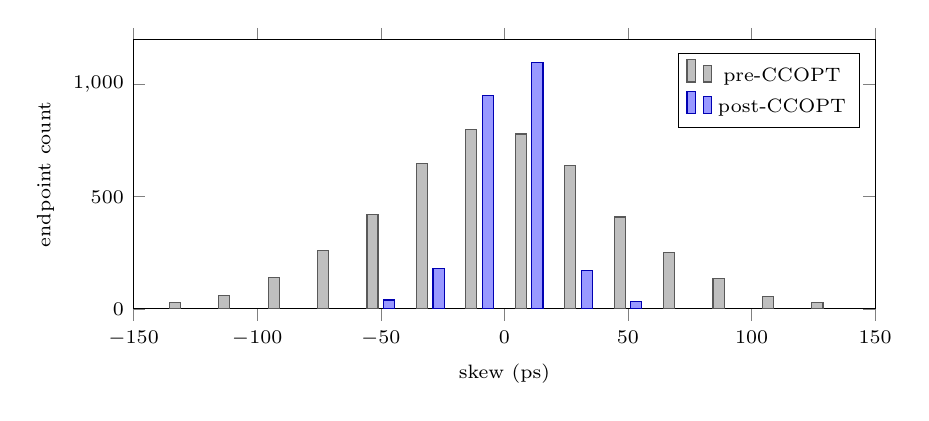
\begin{tikzpicture}
\begin{axis}[
  width=11cm, height=5cm,
  ybar, bar width=4pt,
  xlabel={skew (ps)}, ylabel={endpoint count},
  xmin=-150, xmax=150,
  ymin=0, ymax=1200,
  legend style={font=\scriptsize, at={(0.98,0.95)}, anchor=north east},
  tick label style={font=\scriptsize},
  label style={font=\scriptsize},
]
\addplot+[fill=gray!50, draw=gray!70!black] coordinates {
  (-130,30) (-110,60) (-90,140) (-70,260) (-50,420) (-30,650) (-10,800)
  (10,780) (30,640) (50,410) (70,250) (90,135) (110,55) (130,28)
};
\addlegendentry{pre-CCOPT}
\addplot+[fill=blue!40, draw=blue!70!black] coordinates {
  (-50,40) (-30,180) (-10,950) (10,1100) (30,170) (50,35)
};
\addlegendentry{post-CCOPT}
\end{axis}
\end{tikzpicture}
\caption{Endpoint skew distribution before and after \texttt{ccopt\_design} on a representative block. Pre-CTS the skew spread is essentially the placement-derived latency mismatch (often $\pm$130~ps). Post-CCOPT the distribution collapses to within the spec'd target skew (here 50~ps).}
\label{fig:skew-histogram}
\end{figure}

\begin{pdnote}{Why PD Cares}
\begin{itemize}
  \item \textbf{Arm Duc, your job right now.} Duc CTS work means you are reading CCOPT logs every day; understanding NDR enforcement order is the difference between debugging a clock spine in 20 minutes vs 2 hours. Same for skew groups: a generated clock dropped from the wrong group will produce cross-domain timing failures that look like SDC bugs and are actually a one-line CCOPT spec fix.
  \item \textbf{General PD engineer.} CTS is the only step where the tool builds new logic (clones buffers, inverters, gates) without you naming them in RTL. The spec is the contract that governs that creation; everything you do upstream (placement, floorplan) and downstream (route, sign-off) is reacting to what CCOPT decided.
  \item \textbf{VLSI interview.} ``What is useful skew, and when is it dangerous?'' is asked in roughly half of physical-design interviews. So is ``how do skew groups interact with generated clocks?'' Memorize the worked examples in this chapter and you will outscore most candidates.
\end{itemize}
\end{pdnote}

\begin{checkpoint}
You should now be able to (a) open a CCOPT spec and explain every \texttt{set\_ccopt\_property} line, (b) decide which clocks share a skew group and which do not, (c) compute the M5 track cost of a 2W2S NDR, (d) trade setup against hold with useful skew on a numerical path, and (e) know when mesh is worth its power bill.

\mnemonic{Spec the skew, shield the spine, borrow the slack.}
\end{checkpoint}
